\documentclass[a4paper]{article}
\usepackage[affil-it]{authblk}
\usepackage[backend=bibtex,style=numeric]{biblatex}
\usepackage{amsmath, amsthm, amssymb, amsfonts}
\usepackage{graphicx}
\usepackage{subcaption}
\usepackage{multirow}
\usepackage{hyperref}
\usepackage{cleveref}
\hypersetup{
    colorlinks=true,    % 彩色链接
    linkcolor=blue,      % 内部链接的颜色
    citecolor=red,      % 引用的颜色
    urlcolor=cyan       % 外部链接的颜色
}
\usepackage{geometry}
\usepackage[lined, ruled]{algorithm2e}
\geometry{margin=1.5cm, vmargin={0pt,1cm}}
\setlength{\topmargin}{-1cm}
\setlength{\paperheight}{29.7cm}
\setlength{\textheight}{25.3cm}

\crefname{algorithm}{Algorithm}{Algorithms}
\Crefname{algorithm}{Algorithm}{Algorithms}
\crefname{equation}{Equation}{Equations}
\Crefname{equation}{Equation}{Equations}
\crefname{figure}{Figure}{Figures}
\Crefname{figure}{Figure}{Figures}
\crefname{table}{Table}{Tables}
\Crefname{table}{Table}{Tables}

\crefalias{algocf}{algorithm}

\renewcommand\arraystretch{1.8}

\addbibresource{citation.bib}

\begin{document}
% =================================================
\title{\textbf{Numerical Analysis Programming Report \# 2}}

\author{Haowei Peng 3220104816
  \thanks{E-mail address: \texttt{3220104816@zju.edu.cn}}}
\affil{(Information and Computing Science), Zhejiang University} 

\date{Due time: \today}

\maketitle

\begin{abstract}
    In this programming assignment, we concentrate on the interpolation three different methods. 
    Our basic idea is to find a polynomial that fits the given data points as closely as possible. 
    We will use \textbf{Newton formula, Hermite interpolation, and Bezier curve} to do this.
\end{abstract}

\section*{A. Interpolation.h}

This is the header file for the interpolation program. It contains the following functions and structure:
\begin{itemize}
    \item \verb|long long factorial(int n)|
    \item \verb|long long combination(int n, int k)|
    \item \verb|struct Point|
\end{itemize}

and the following classes:

\begin{itemize}
    \item \verb|Polynomial|
    \item \verb|Curve|
    \item \verb|Interpolation|
    \begin{itemize}
        \item \verb|Newton_Interpolation|
        \item \verb|Hermite_Interpolation|
        \item \verb|Bezier_Curve|
    \end{itemize}
\end{itemize}

\subsection*{A.1 Functions}

\subsubsection*{A.1.1 factorial}

This function calculates the factorial of a given integer $n$, i.e. $n!$.

\subsubsection*{A.1.2 combination}

This function calculates the combination of $n$ objects taken $k$ at a time, i.e. 
\begin{equation}
    \binom{n}{k} = \frac{n!}{k!(n - k)!}.
    \label{eq:combination}
\end{equation}

\subsection*{A.2 Structure}

\subsubsection*{A.2.1 Point}

This structure represents a point. The parameters' meanings follow
\begin{itemize}
    \item \verb|double x|: the x-coordinate of the point
    \item \verb|int order|: the order of the point
    \item \verb|double *f|: the function values at the point
\end{itemize}

\subsection*{A.3 Classes}

\subsubsection*{A.3.1 Polynomial}

This class has two member variables \verb|std::vector<double> coeff| and \verb|std::vector<Point> points|, which means the coefficients of the polynomial and the data points, respectively.

And it has two member functions, calculating the value and derivative of the point $x$. The calculation of derivative uses the formula
\begin{equation}
    (f_1(x)f_2(x) \cdots f_n(x))' = \sum_{i = 1}^n \left(f'_i(x) \cdot \prod_{j = 1, j \neq i}^n f_j(x)\right).
    \label{eq:derivative}
\end{equation}

\subsubsection*{A.3.2 Curve}

This class is similar to \verb|Polynomial|, while it only has one member variable \verb|std::vector<long long> coeff|.

\subsubsection*{A.3.3 Interpolation}

This class is the base class for all interpolation methods. It has one member variable \verb|std::vector<Point> points| and one member function \verb|Interpolation(std::vector<Point> points)|, which initializes the data points.

\subsubsection*{A.3.4 Newton\_Interpolation, Hermite\_Interpolation, Bezier\_Curve}

These classes are derived from \verb|Interpolation|, and they implement the corresponding interpolation methods.

The algorithms are illustrated in the \cref{alg:Newton,alg:Hermite,alg:Bezier}.

\subsection*{A.4 The algorithms used in the header file}

\subsubsection*{A.4.1 The Newton formula}

Firstly we need to give a definition of symmetric polynomials 
\begin{equation}
    \pi_n(x) = \begin{cases}
        1, & n = 0; \\
        \prod_{i = 0}^{n - 1} (x - x_i), & n > 0.
    \end{cases}
    \label{eq:sym_poly}
\end{equation}

The Newton formula for interpolating the values $f_0, f_1, \cdots, f_n$ at distinct points $x_0, x_1, \cdots, x_n$ is 
\begin{equation}
    p_n(x) = \sum_{k = 0}^n a_k \pi_k(x),
    \label{eq:Newton}
\end{equation}
where $\pi_k(x)$ is defined in \cref{eq:sym_poly} and $a_k$ is the divided difference denoted by $f[x_0, x_1, \cdots, x_k]$.

The divided difference can be defined by induction as 
\begin{equation}
    \begin{aligned}
        f[x_0] & = f(x_0), \\
        f[x_0, x_1] & = \frac{f[x_1] - f[x_0]}{x_1 - x_0} = \frac{f(x_1) - f(x_0)}{x_1 - x_0}, \\ 
        f[x_0, x_1, x_2] & = \frac{f[x_1, x_2] - f[x_0, x_1]}{x_2 - x_0}, \\
        & \vdots \\
        f[x_0, x_1, \cdots, x_k] & = \frac{f[x_1, \cdots, x_k] - f[x_0, \cdots, x_{k-1}]}{x_k - x_0}. \\
    \end{aligned}
    \label{eq:div_diff}
\end{equation}

So the Newton interpolation algorithm can be shown as follows.

\begin{algorithm}[H]
    \KwIn{$x_0, f_0, x_1, f_1, \cdots, x_n, f_n.$}
    \KwOut{$a_0, a_1, \cdots, a_{n - 1}.$}
    \BlankLine
    \For{$i = 0, 1, \cdots, n - 1$}{
        \For{$j = 0, 1, \cdots, i$}{
            $d_{i, j} \leftarrow \frac{d_{i, j - 1} - d_{i - 1, j - 1}}{x_i - x_{i - j}}$ \;
        }
        $a_i \leftarrow d_{i, i}$\;
    }
    \caption{the Newton interpolation algorithm}
    \label{alg:Newton}
\end{algorithm}

\subsubsection*{A.4.2 The Hermite interpolation}

The Hermite interpolation method is similar to the Newton interpolation method, but it takes the derivative into consideration.

In this section, \cref{eq:div_diff} changes to the generalized divided difference. 
The generalized divided difference takes the order of the derivative into consideration. This algorithm is illustrated in \cref{alg:Hermite}.

\begin{algorithm}[H]
    \KwIn{$x_0, f_0, f'_0, \cdots, f_0^{(m_0)}, x_1, f_1, \cdots, f_1^{(m_1)}, \cdots, x_n, f_n, f'_n, \cdots, f_n^{(m_n)}.$}
    \KwOut{$a_0, a_1, \cdots, a_{N - 1}, \quad N := k + \sum_{i = 0}^k m_i.$}
    \BlankLine
    \For{$i = 0, 1, \cdots, N - 1$}{
        \For{$j = 0, 1, \cdots, i$}{
            \uIf{$x_i \ne x_j$} {
                $d_{i, j} \leftarrow \frac{d_{i, j - 1} - d_{i - 1, j - 1}}{x_i - x_{i - j}}$ \;
            }
            \Else{
                $d_{i, j} \leftarrow \frac{f_i^{(i - j)}}{(i - j)!}$ \;
            }
        }
        $a_i \leftarrow d_{i, i}$\;
    }
    \caption{the Hermite interpolation algorithm}
    \label{alg:Hermite}
\end{algorithm}

\subsubsection*{A.4.3 The Bezier curve}

Firstly we introduce the Bernstein polynomials. The Bernstein polynomials of degree $n \in \mathbb{N}^+$ relative to the unit interval $[0, 1]$ are
\begin{equation}
    \forall k = 0, 1, \cdots, n, \quad b_{n, k}(t) = \binom{n}{k} t^k (1 - t)^{n - k},
    \label{eq:bernstein}
\end{equation}
and $b_{n, k}(t) = 0$ for all other values of the integer $k$.

The Bezier curve of $n + 1$ distinct points $\mathbf{q}_0, \mathbf{q}_1, \cdots, \mathbf{q}_n$ in $\mathbb{R}^D$ is the curve $\mathbf{B}: [0, 1] \rightarrow \mathbb{R}^D$ given by
\begin{equation}
    \mathbf{B}(t) := \sum_{k = 0}^n \mathbf{q}_k b_{n, k}(t),
    \label{eq:bezier}
\end{equation}
where $n \in \mathbb{N}^+$, $b_{n, k}$ is the $k$-th Bernstein polynomial of degree $n$ in \cref{eq:bernstein}. 
The points $\mathbf{q}_k$'s are called the \textit{control points}. 

For the tangent vector, we define it as the first derivative 
\begin{equation}
    \gamma' := \frac{\mathrm{d}\gamma}{\mathrm{d}t}
    \label{eq:tangent_vector}
\end{equation}
and the unit tangent vector of $\gamma$, denoted by $\mathbf{t}$.

The Bezier curve-fitting algorithm is illustrated in \cref{alg:Bezier}.

\begin{algorithm}[H]
    \KwIn{$m + 1$ consecutive marker points $\mathbf{p}_0, \cdots, \mathbf{p}_m$ on $\gamma$}
    \KwOut{The Bezier curve $\mathbf{B_{\mathrm{result}}}$}
    \BlankLine
    \For{$j = 0, 1, \cdots, m - 1$}{
        $\mathbf{q_0} \leftarrow \mathbf{p}_j$ \;
        $\mathbf{q_1} \leftarrow \frac{1}{3}\gamma'(\mathbf{p}_j) + \mathbf{p}_j$ \;
        $\mathbf{q_2} \leftarrow \mathbf{p}_{j + 1} - \frac{1}{3}\gamma'(\mathbf{p}_j)$ \;
        $\mathbf{q_3} \leftarrow \mathbf{p}_{j + 1}$ \;
        $\mathbf{B}_j \leftarrow \mathbf{B}(\mathbf{q}_0, \mathbf{q}_1, \mathbf{q}_2, \mathbf{q}_3)$ \;
    }
    $\mathbf{B}_{\mathrm{result}} \leftarrow \sum_{j = 0}^{m - 1} \mathbf{B}_j$ \;
    \caption{the Bezier curve-fitting algorithm}
    \label{alg:Bezier}
\end{algorithm}

\section*{B. Interpolate the Runge function by Newton interpolation}

In this section, we need to interpolate the function 
\begin{equation}
    f(x) = \frac{1}{1 + x^2}
    \label{eq:B.runge}
\end{equation}
for $x \in [-5, 5]$ using $x_i = -5 + 10\frac{i}{n},\ i = 0, 1, \cdots, n$, and $n = 2, 4, 6, 8$.

The results are shown as follows:

\begin{figure}[htbp]
    \centering
    \begin{subfigure}[b]{0.48\textwidth}
        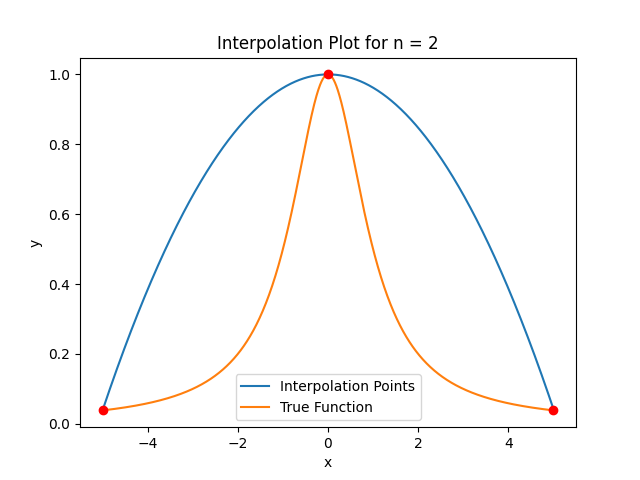
\includegraphics[width=\textwidth]{../results/Task_B/Interpolation_Plot_n_2.png}
        \caption{Interpolation result for $n = 2$}
    \end{subfigure}
    \hfill
    \begin{subfigure}[b]{0.48\textwidth}
        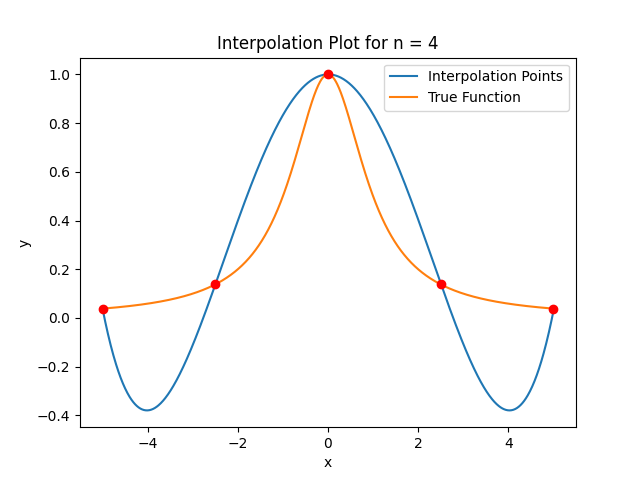
\includegraphics[width=\textwidth]{../results/Task_B/Interpolation_Plot_n_4.png}
        \caption{Interpolation result for $n = 4$}
    \end{subfigure}

    \begin{subfigure}[b]{0.48\textwidth}
        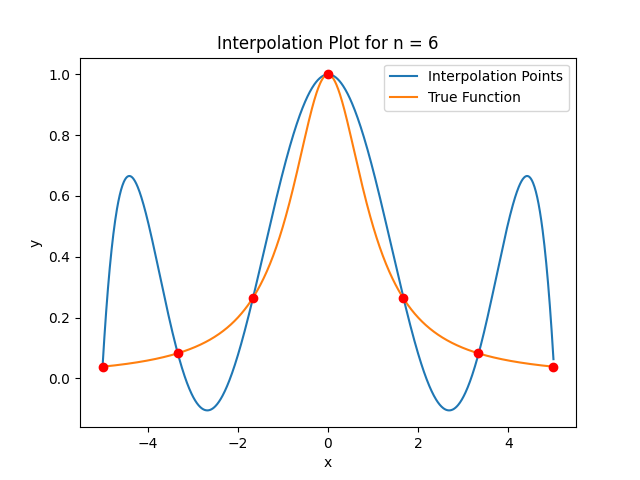
\includegraphics[width=\textwidth]{../results/Task_B/Interpolation_Plot_n_6.png}
        \caption{Interpolation result for $n = 6$}
    \end{subfigure}
    \hfill
    \begin{subfigure}[b]{0.48\textwidth}
        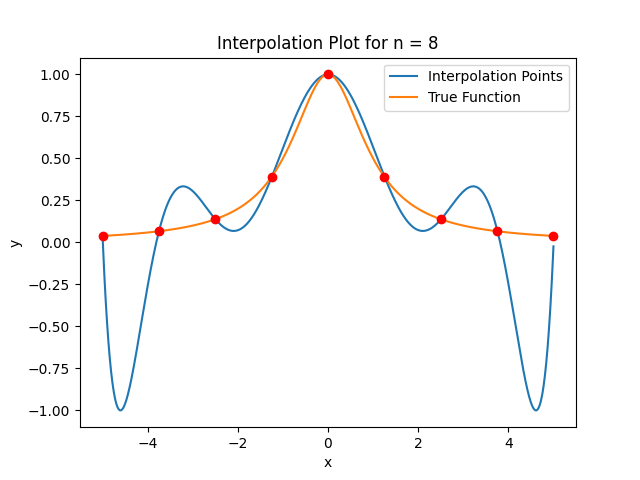
\includegraphics[width=\textwidth]{../results/Task_B/Interpolation_Plot_n_8.png}
        \caption{Interpolation result for $n = 8$}
    \end{subfigure}
    \caption{Interpolation results for $n = 2, 4, 6, 8.$}
    \label{fig:B.results}
\end{figure}

From \cref{fig:B.results}, we can find that the interpolation function oscillates more obviously as $n$ increases, which implies the Runge phenomenon.

\section*{C. Interpolate another function on the zeros of Chebyshev polynomials}

In this section, we need to interpolate the function 
\begin{equation}
    f(x) = \frac{1}{1 + 25x^2},
    \label{eq:C.chebyshev}
\end{equation}
which is similar to \cref{eq:B.runge}.

According to the Theorem 2.45 in our textbook, the zeros of the Chebyshev polynomials $T(n)$ are
\begin{equation}
    x_k = \cos \frac{2k - 1}{2n}\pi,
    \label{eq:C.zeros}
\end{equation} 

and we interpolate \cref{eq:C.chebyshev} in the \cref{eq:C.zeros} with $n = 5, 10, 15, 20$.
The results are shown as \cref{fig:C.results}.

\begin{figure}[htbp]
    \centering
    \begin{subfigure}[b]{0.48\textwidth}
        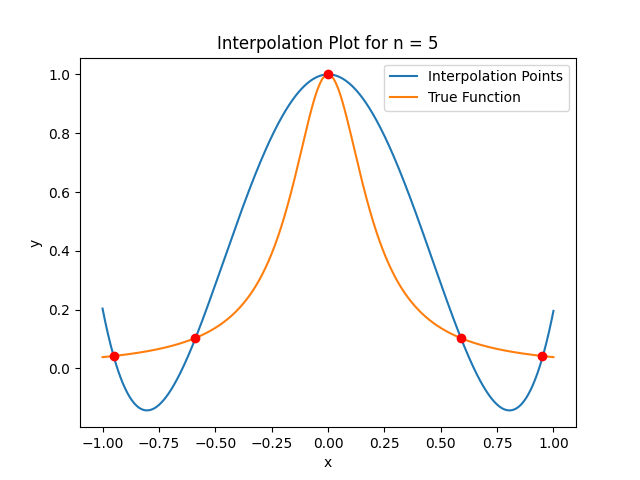
\includegraphics[width = \textwidth]{../results/Task_C/Interpolation_Plot_n_5.png}
        \caption{Interpolation result for $n = 5$}
    \end{subfigure}
    \hfill
    \begin{subfigure}[b]{0.48\textwidth}
        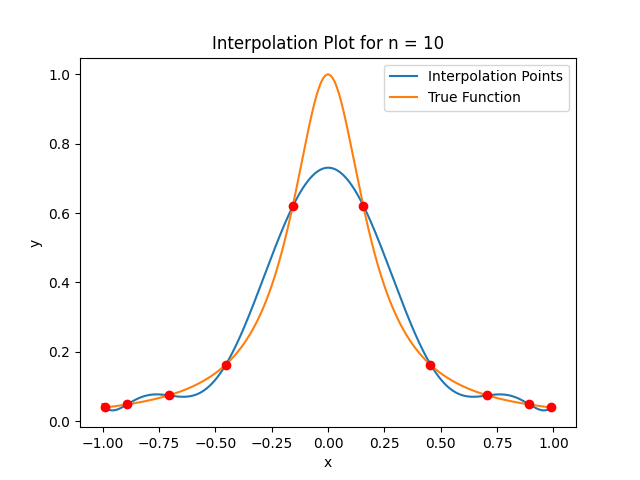
\includegraphics[width = \textwidth]{../results/Task_C/Interpolation_Plot_n_10.png}
        \caption{Interpolation result for $n = 10$}
    \end{subfigure}

    \begin{subfigure}[b]{0.48\textwidth}
        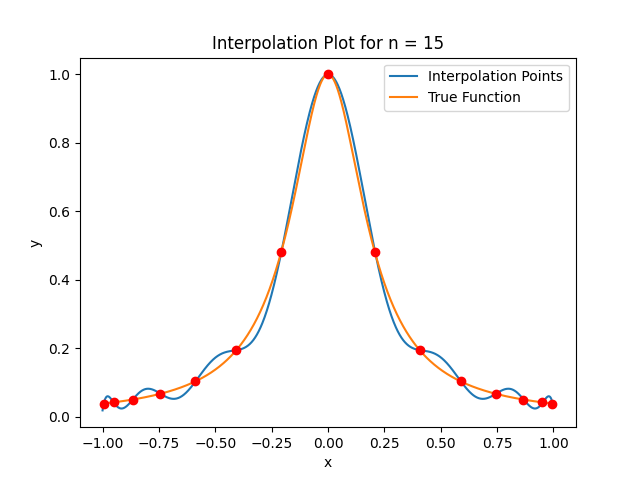
\includegraphics[width = \textwidth]{../results/Task_C/Interpolation_Plot_n_15.png}
        \caption{Interpolation result for $n = 15$}
    \end{subfigure}
    \hfill
    \begin{subfigure}[b]{0.48\textwidth}
        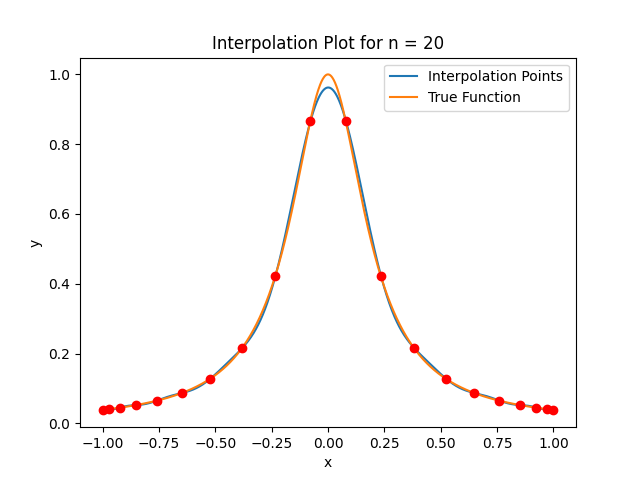
\includegraphics[width = \textwidth]{../results/Task_C/Interpolation_Plot_n_20.png}
        \caption{Interpolation result for $n = 20$}
    \end{subfigure}

    \begin{subfigure}[b]{0.48\textwidth}
        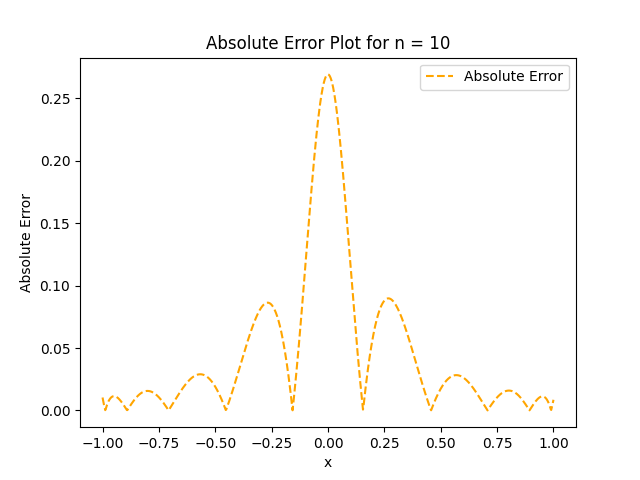
\includegraphics[width = \textwidth]{../results/Task_C/Absolute_Error_Plot_n_10.png}
        \caption{Absolute error for $n = 10$}
    \end{subfigure}
    \hfill
    \begin{subfigure}[b]{0.48\textwidth}
        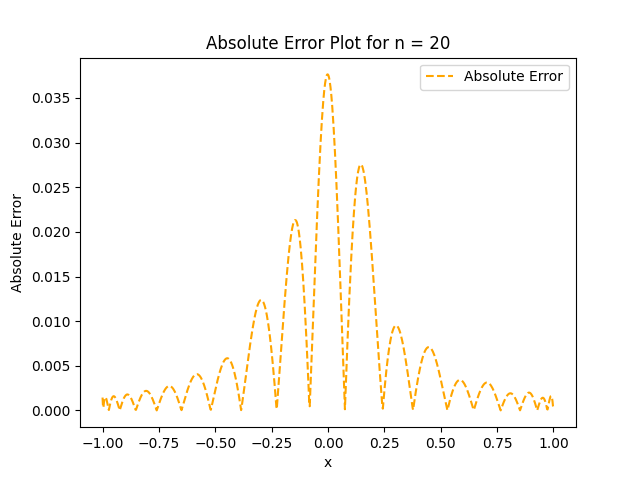
\includegraphics[width = \textwidth]{../results/Task_C/Absolute_Error_Plot_n_20.png}
        \caption{Absolute error for $n = 20$}
    \end{subfigure}

    \caption{Interpolation results for $n = 5, 10, 15, 20$, and the absolute error for $n = 10, 20.$}
    \label{fig:C.results}
\end{figure}

Obviously we can know that the Runge phenomenon is smaller than the pure Newton interpolation, and the absolute error goes to smaller as $n$ increases, which shows that the Chebyshev interpolation is free of the wide oscillations in the previous assignments.

\section*{D. Interpolate a function using Hermite interpolation}

In this section, we need to interpolate a function of position and velocity.

The given data points are
\begin{table}[htbp]
    \centering 
    \renewcommand{\arraystretch}{0.95}
    \begin{tabular}{|c|c|c|c|c|c|}
        \hline 
        Time & 0 & 3 & 5 & 8 & 13 \\
        \hline
        Position & 0 & 225 & 383 & 623 & 993 \\
        \hline
        Velocity & 75 & 77 & 80 & 74 & 72 \\
        \hline
    \end{tabular}
    \caption{Data points for the position and velocity of the car}
    \label{tab:D.data}
    \renewcommand{\arraystretch}{1.0}
\end{table}

And the position of the car and its speed for $t = 10$ seconds are
\begin{equation}
    x = 742.5028\ \mathrm{feet}, \quad v = 48.3814\ \mathrm{feet/s},
    \label{eq:D.hermite}
\end{equation}

while the maximum speed is $v_{\mathrm{max}} = 119.4160\ \mathrm{feet/s}$, so the car ever exceeds the speed limit.

\section*{E. Interpolate the weight function by Newton's formula}

The data given is 
\begin{table}[htbp]
    \centering
    \renewcommand{\arraystretch}{0.95}
    \begin{tabular}{|c|c|c|c|c|c|c|c|}
        \hline
        Day & 0 & 6 & 10 & 13 & 17 & 20 & 28 \\
        \hline
        Sp1 & 6.67 & 17.3 & 42.7 & 37.3 & 30.1 & 29.3 & 28.7 \\
        \hline 
        Sp2 & 6.67 & 16.1 & 18.9 & 15.0 & 10.6 & 9.44 & 8.89 \\
        \hline        
    \end{tabular}
    \caption{Data points for the average weight of two species}
    \label{tab:E.data}
    \renewcommand{\arraystretch}{1.0}
\end{table}

The interpolation result is shown as follows in \cref{fig:E.result}.

\begin{figure}[htbp]
    \centering
    \begin{subfigure}[b]{0.45\textwidth}
        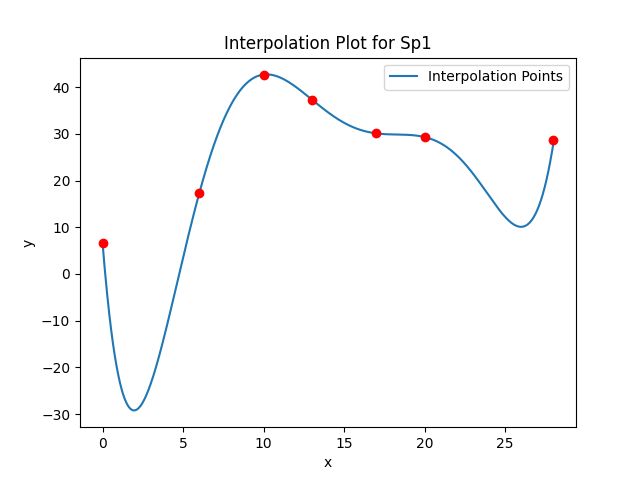
\includegraphics[width=\textwidth]{../results/Task_E/Interpolation_Plot_Sp1.png}
        \caption{Interpolation result for species 1}
    \end{subfigure}
    \hfill
    \begin{subfigure}[b]{0.45\textwidth}
        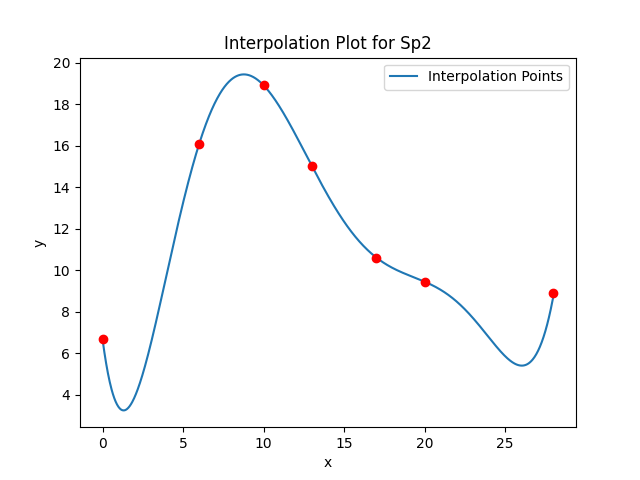
\includegraphics[width=\textwidth]{../results/Task_E/Interpolation_Plot_Sp2.png}
        \caption{Interpolation result for species 2}
    \end{subfigure}
    \caption{Interpolation results for species 1 and 2}
    \label{fig:E.result}
\end{figure}

And for the weight after another 15 days, we predict
\begin{equation}
    x_1 = 14640.2578, \quad x_2 = 2981.4769,
    \label{eq:E.predict}
\end{equation}
where $x_1, x_2$ is the average weight of species 1 and 2, respectively. So no sample of larvae will die after 15 days.

\section*{F. Approximate a closed planar curve in the shape of a heart by Bezier curves}

In this section, we need to approximate a closed planar curve with $m = 10, 40, 160$ in \cref{alg:Bezier}.
The given function is 
\begin{equation}
    x^2 + (\frac{3}{2}y - \sqrt{|x|})^2 = 3,
    \label{eq:F.heart}
\end{equation}
and its roots constitute a closed planar curve in the shape of a heart.

The characteristic points of the heart are 
\begin{equation}
    P_0(0, \frac{2}{\sqrt{3}}),\ P_1(\sqrt{3}, \frac{2}{3} \sqrt[4]{3}),\ P_2(\frac{\sqrt{13} - 1}{2}, 0),\ P_3(0, -\frac{2}{\sqrt{3}}),\ P_4(\frac{1 - \sqrt{13}}{2}, 0),\ P_5(-\sqrt{3}, \frac{2}{3} \sqrt[4]{3}),
    \label{eq:F.heart_points}
\end{equation}
then the whole curve can be divided into six parts $C_0, \cdots, C_5$.

The \cref{eq:F.heart} can be rewritten as 
\begin{equation}
    y = 
    \begin{cases}
        f_1(x) = \frac{2}{3} (\sqrt{|x|} + \sqrt{3 - x^2}), & y \geqslant \frac{2}{3} \sqrt[4]{3}, \\
        f_2(x) = \frac{2}{3} (\sqrt{|x|} - \sqrt{3 - x^2}), & y < \frac{2}{3} \sqrt[4]{3}, \\
    \end{cases}
    \label{eq:F.heart_rewrite}
\end{equation}
and we use $f_1$ in the upper part ($C_0, C_5$) and use $f_2$ in the lower part ($C_1, C_2, C_3, C_4$).

The results of the approximation are shown as follows in \cref{fig:F.results}.

\begin{figure}[htbp]
    \centering
    \begin{subfigure}[b]{0.32 \textwidth}
        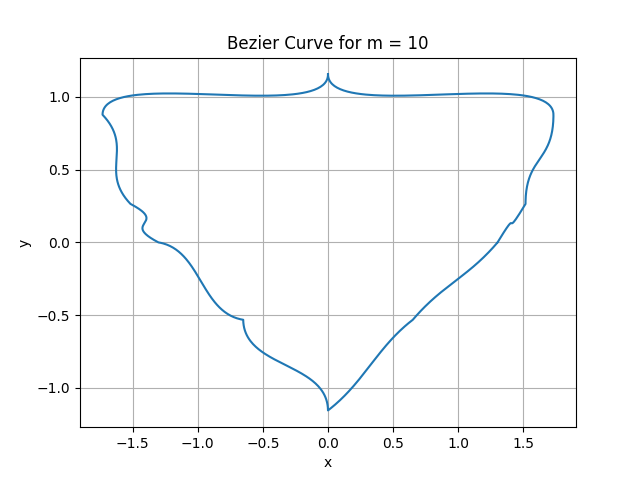
\includegraphics[width=\textwidth]{../results/Task_F/Task_F_m_10.png}
        \caption{$m = 10$}
    \end{subfigure}
    \hfill
    \begin{subfigure}[b]{0.32 \textwidth}
        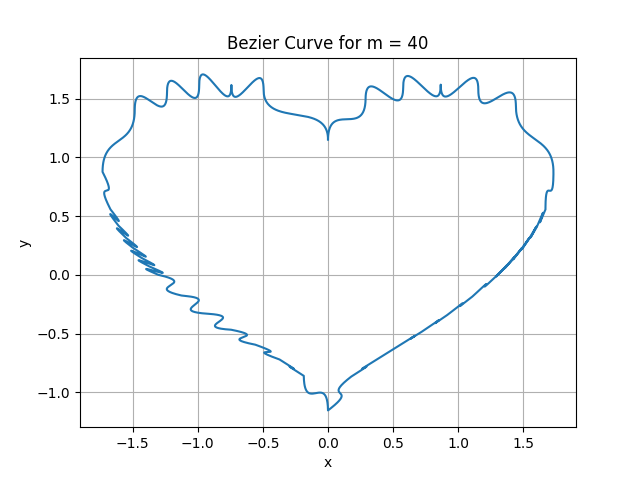
\includegraphics[width=\textwidth]{../results/Task_F/Task_F_m_40.png}
        \caption{$m = 40$}
    \end{subfigure}
    \hfill
    \begin{subfigure}[b]{0.32 \textwidth}
        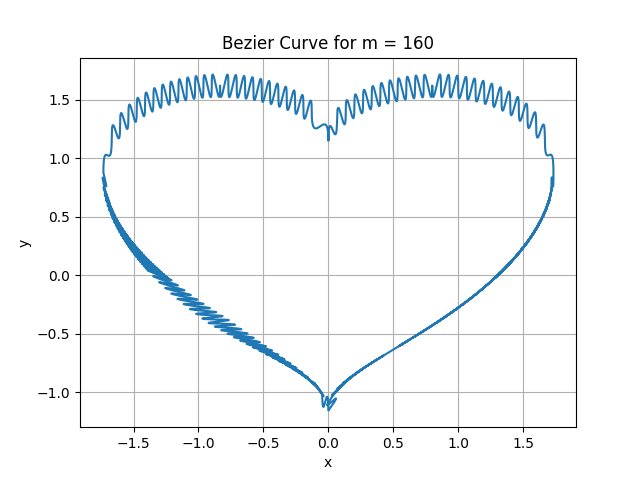
\includegraphics[width=\textwidth]{../results/Task_F/Task_F_m_160.png}
        \caption{$m = 160$}
    \end{subfigure}
    \caption{Approximation results for $m = 10, 40, 160.$}
    \label{fig:F.results}
\end{figure}

As $m$ increases, the approximation becomes more accurate, and the shape of the heart becomes more like a heart.

\section*{\center{\normalsize {Ackonwledgement}}}

Above all, I would like to apologize sincerely for the late submission of this assignment. 
The task F spends me plenty of time to finish, so I have to hand in my assignment after five days of the deadline.

In the process of finishing the task, I get help from \href{https://kimi.moonshot.cn}{\textit{Kimi AI}}, which tells me how to fix some mistakes in the code and report.

\end{document}